\documentclass{beamer}
%[aspectratio=169]   \usepackage[czech]{babel}
\usepackage{apo-lecture-en}
\usepackage{pdfpages}
\usepackage{pdfcomment}
\usepackage{listings}
\usepackage{array,multirow}
\usepackage{environ}

\subtitle{Lecture 09. External Events Processing}
\author{Pavel Píša \phantom{xxxxxxxxx} Petr Štěpán \\ \small\texttt{pisa@fel.cvut.cz}\phantom{xxxx}\small\texttt{stepan@fel.cvut.cz}}

\begin{document}

\maketitle

\section{Computer Use Areas/Connections With the Real World}

\begin{frame}
\frametitle{Today's Lecture Objective}

\begin{itemize}
 \item Computer use areas/connection to the real world
 \item Peripheral handling and impact on processor load
 \item Event handling, interrupts and exceptions
 \item Direct memory access from peripherals
 \item Consequences of using cache memories, out-of-order processing, multiple processors
\end{itemize}
\end{frame}

\begin{frame}
\frametitle{Review of previously discussed building blocks}

\begin{itemize}
 \item Central Processing Unit (CPU)
 \item Memory -- for data and code ordered into hierarchy
 \begin{itemize}
  \item Registers (fast CPU local memory)
  \item Cache (L1, L2, etc)
  \item Main memory (RAM -- DDR most used today)
  \item Externalmemory /secondary storage (disks, Flash)
 \end{itemize}
 \item Interconnection -- buses, networking
 \begin{itemize}
  \item ISA, PCI, PCIexpress, AXI
 \end{itemize}
\end{itemize}
\end{frame}

\begin{frame}
\frametitle{Areas, Where Introduced Blocks, Processors Are Used}

\begin{itemize}
 \item Entertainment
 \begin{itemize}
  \item historically the first sequential machines, automaton - music boxes, clocks, astronomical clocks, Antikythera mechanism as early as 150 BC.
  \item today slot machines, game consoles, simulators, multimedia
 \end{itemize}
 \item Enterprise, bank, accountancy, inventory, online shops
 \begin{itemize}
  \item originally only adding machines, cash registers, today stock exchanges, enterprise (ERP, SCM, CRM) and banking information systems, etc.
 \end{itemize}
 \item Large scale mathematical and modeling computation
 \begin{itemize}
  \item global climatic forecast and analysis, nuclear fusion, etc.
  \item machine learning
 \end{itemize}
 \item Communications
 \begin{itemize}
  \item as the main purpose networking hardware, originally landline telephone, mobile
  \item as the indivisible component of all other applications
 \end{itemize}
 \item Automation, production, transport
 \begin{itemize}
  \item originally automatic patterns loom, today welding, robotics, autonomous cars and trains
 \end{itemize}
 \item and many other areas
\end{itemize}
\end{frame}

\begin{frame}
\frametitle{Computer in Control Applications}

\begin{columns}
\begin{column}{0.58\textwidth}
Replaces single/specific purpose controllers. Advantages:
\begin{enumerate}
 \item often complex equations, math, rules, relationships
 \begin{itemize}
  \item fast calculation
 \end{itemize}
 \item cheap due to serial production
 \item very flexible
 \begin{itemize}
  \item programmable, reusable
 \end{itemize}
 \item precise/deterministic processing of (physical) quantities
 \begin{itemize}
  \item values reprezentationa and limits
 \end{itemize}
 \item hierarchical control
 \begin{itemize}
  \item is easier, possible
 \end{itemize}
 \item complex algorithms
 \begin{itemize}
  \item only memory and time limitations
 \end{itemize}
\end{enumerate}
  \vfil
\end{column}
\begin{column}{0.42\textwidth}
  \begin{center}
    Computer as control system

    \vspace{5mm}

    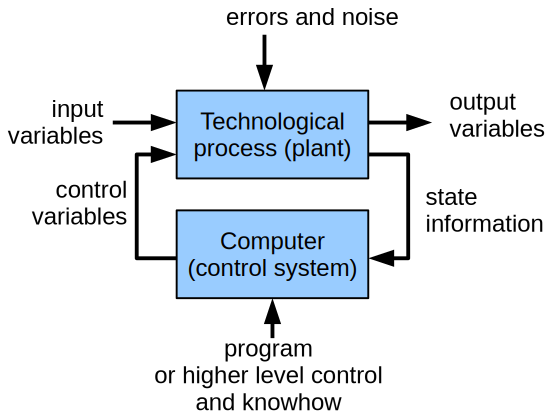
\includegraphics[width=1.0\textwidth]{computer-as-controller-en.pdf}
  \end{center}
\end{column}
\end{columns}
\end{frame}

\begin{frame}
\frametitle{Various Requirements for Processing Tasks, Data}

\begin{itemize}
 \item Batch processing
 \begin{itemize}
  \item the task accesses data as it needs them for processing and the timing and order of output corersponds to computations order
 \end{itemize}
 \item Interactive
 \begin{itemize}
  \item usually event driven. Requests, inputs from the user or from another system are initial events
 \end{itemize}
 \item Real-time control (of technologies, robots, cars)
 \begin{itemize}
  \item even the most accurate outputs delivered late have no value (the plane has already crashed) or value is significantly reduced (tears in video transmission)
  \item hard real-time/soft real-time
  \item Safety Integrity Level (SIL) if there is a risk of harm to health and property
 \end{itemize}

\end{itemize}
\end{frame}

\section{Peripherals Access and Drivers}

\begin{frame}
\frametitle{Input/Output Subsystem (from Lecture 8.)}

\begin{itemize}
 \item Input-only peripherals
 \begin{itemize}
  \item common: keyboard, mouse, video camera
  \item digital inputs, physical quantities -- usually converted to analog
electrical signal and then by an A/D converter to a digital representation
accessible on an input port, or directly to to logical (0/1) or its change in time
 \end{itemize}
\end{itemize}
\begin{itemize}
 \item Output-only peripherals
 \begin{itemize}
  \item video output (2D, 3D + acceleration), audio output
  \item outputs with physical effects, 3D printer (rapid prototyping),
process control (D/A converters, PWM) and many
other types of drives
 \end{itemize}
\end{itemize}
\begin{itemize}
 \item Bidirectional communication
 \begin{itemize}
  \item hard disk, NVME Flash, communication interfaces
  \item most of the above "unidirectional" peripherals require read
and write access for their settings, monitoring and parameters
control
 \end{itemize}
\end{itemize}
\end{frame}

\begin{frame}
\frametitle{Methods to Transfer Data between Peripherals and CPU}

\begin{itemize}
 \item Programmed input/output (PIO) with polling
 \begin{itemize}
  \item CPU loops in cycle and waits for status information signaling
        available input data or space in output buffer
 \end{itemize}
\end{itemize}
\begin{itemize}
 \item Interrupt driven programmed input/output (PIO)
 \begin{itemize}
  \item processor/program/operating system configures peripheral but does not wait
        for data. Data arrival is signaled by interrupt (asynchronous
        event/exception). The data are read in interrupt service
        routine.
  \item output is initiated by CPU write of data to a register if space
        is available. Ready for next data it signaled by interrupt.
 \end{itemize}
\end{itemize}
\begin{itemize}
 \item Direct memory access (DMA)
 \begin{itemize}
  \item processor/program/operating system setups the source and destination,
        the transfer is carried out by a specialized unit, completion is signaled
        by an interrupt.
 \end{itemize}
\end{itemize}
\begin{itemize}
 \item Intelligent peripherals/controllers
 \begin{itemize}
  \item the operation even with transfers to/from memory (bus master -- DMA)
 \end{itemize}
\end{itemize}
\end{frame}

\section{Events Processing, Interrupts and Exceptions}

\begin{frame}
\frametitle{The Main Instruction Cycle of the CPU (from Lecture 3.)}
\begin{enumerate}
  \item Initial setup/reset -- set initial PC value, PSW, etc. after power-up or processor reset
  \item Read the instruction from the memory
  \begin{itemize}
    \item $PC \to$ to the address bus
    \item Read the memory contents (machine instruction) and transfer it to $IR$
    \item $PC+l \to PC$, point $PC$ to next instruction, $l$ is length of actually processed instruction
  \end{itemize}
  \item Decode operation code (opcode)
  \item Execute the operation
  \begin{itemize}
    \item compute effective address, select registers, read operands, pass them through ALU and store result
  \end{itemize}
  \item Check for exceptions/interrupts (and service them)
  \begin{itemize}
    \item if the exception is a result of executing the given instruction, ensure that its outputs are not stored and $PC$ continues to point to it
    \item set $PC$ to start of the service routine/IRQ handler. Store previous $PC$ and enough of CPU state so that it is possible to continue the interrupted instruction sequence after return from the handler 
  \end{itemize}
  \item Repeat from the step 2
\end{enumerate}
\end{frame}


\begin{frame}
\frametitle{Exceptions and Interrupts}

\begin{itemize}
 \item Exceptions (synchronous) -- anomalous or exceptional situations (blocking
further regular execution) requiring special processing
 \item Main causes:
 \begin{itemize}
  \item Undefined instruction (RISC V -- unknown opcode)
  \item Arithmetic exception (divide by zero, overflow -- on RISC-V does not exist for integer unit, for floating point yes)
  \item System call (activated by system call instruction -- syscall)
  \item Data unavailable or read/write fault or bus error
  \item Bad address or page marked as not-presnet, invalid, protected, etc.
  \item Instruction forbidden for given processor mode (user, system, machine)
  \item Bus error detected (parity, ECC, acknowledge limit exceed)
 \end{itemize}
 \item Asynchronous/external exceptions (interrupts)
 \begin{itemize}
  \item not a direct consequence of the execution of the instruction
  \item usually, it is impossible to determine on the instruction, clock cycle, exactly when the event occured
 \end{itemize}
\end{itemize}
\end{frame}

\begin{frame}
\frametitle{Asynchronous/External Exceptions (Interrupts)}

\begin{itemize}
 \item Maskable, can be disabled in CPU/processor status word -- PSW
 \begin{itemize}
   \item either all or up to a certain priority of resources
   \item peripherals, counters, timers, GPIO events
   \item interprocessor communication, event to other cores that they should take over the task and others
   \item usually maskable also on the peripheral source or controller, optionally also with priority setting
 \end{itemize}
 \item Non-maskable
 \begin{itemize}
  \item hardware failures, supervisory circuits (Watch Dog)
 \end{itemize}
\end{itemize}
\end{frame}

\begin{frame}
\frametitle{Steps of Exception or Interrupt Processing}

\begin{itemize}
 \item An synchronous exception is usually accepted/handled unconditionally,
an external interrupt only if it is not masked or if it is not masked
\end{itemize}

\begin{enumerate}
 \item CPU state vector is saved including $PC$
 \begin{itemize}
  \item to the system stack or to specialized processor registers (ELR, EPC)
  \item how much of the state is stored in the first phase by hardware and how much later by a service routine varies between architectures
  \item when interrupted in user mode, the mode is switched to system (or machine)
  \item usually other interrupts or lower and equal priorities are disabled
 \end{itemize}
 \item The program counter is preset to the starting address of the service routine
 \begin{itemize}
  \item either one for all sources, or depending on the type of exception or even the individual interrupt source number
 \end{itemize}
 \item The service routine starting at this address is executed
 \begin{itemize}
  \item which usually stores the state of other registers used by ISR on the stack, communicates with peripherals, reads the missing page, informs about an unrecoverable error of the task or the entire system, etc.
 \end{itemize}
\end{enumerate}
\end{frame}

\begin{frame}
\frametitle{Steps of Exception or Interrupt Processing -- Final Part}

\begin{enumerate}
 \setcounter{enumi}{4}
 \item If the cause is recoverable -- the routine restores the values ​​of the registers to the state before exception/interrupt invocation
 \begin{itemize}
  \item in the case of systemcall or emulated instruction, some part of the previously saved state is modified to expose the results
 \end{itemize}
 \item The return from the routine is realized by exception return instruction
 \begin{itemize}
  \item this switches the processor to the previous state, including the instruction counter, mode, etc. and allows the continuation of the interrupted code
 \end{itemize}
\end{enumerate}
\begin{itemize}
 \item Then it continues either by restarting the instruction that caused the exception, or by continuing from the next instruction, in the case of an external interrupt, system call, or emulation of an instruction that is not directly supported
\end{itemize}
\end{frame}

\begin{frame}
\frametitle{Exception Sources on the RISC-V Architecture}

\begin{itemize}
 \item Exceptions caused by hardware failure:
 \begin{itemize}
  \item Machine Check: The processor detects an internal inconsistency
  \item Bus Error: when data loading or storing or fetching of an instruction
 \end{itemize}
 \item Exceptions caused by some external (for the processor) causes:
 \begin{itemize}
  \item Reset: A signal activated on the appropriate pin of the package, core
  \item Non-maskable interrupt (NMI): The rising edge of the appropriate signal
 \end{itemize}
 \item Hardware interrupts: Activated by corresponding signals
 \begin{itemize}
  \item Hardware interrupts can be masked by setting the corresponding bits of the status register
 \end{itemize}
 \item Exceptions that occur due to problems with instruction execution
\end{itemize}
\end{frame}

\begin{frame}
\frametitle{Exception Sources on the RISC-V Architecture -- Continuation}

\begin{itemize}
 \item Exceptions that occur due to problems with instruction execution
 \begin{itemize}
  \item Address Error: a reference to an invalid memory area, or a reference to the kernel address space from user mode
 \item Invalid instruction: An undefined opcode field (or privileged
instructions in user mode)
 \end{itemize}
 \item Exceptions caused by the execution of instructions intended for this purpose
 \begin{itemize}
  \item system call (Syscall): \textbf{ecall} executed
  \item debugging/break instruction (Break): \textbf{ebreak} executed
 \end{itemize}
\end{itemize}
\end{frame}

\begin{frame}
\frametitle{RISC-V -- Status and Control Registers Related to Exception Handling}

\begin{tabular}{|l|l|l|}  \hline
Register Name & Number & Description/Use \\\hline
mstatus & 0x300 & Machine status register \\\hline
misa & 0x301 & ISA and extensions \\\hline
mie & 0x304 & Machine interrupt-enable register \\\hline
mtvec & 0x305 & Machine trap-handler base address \\\hline
mscratch & 0x340 &Scratch register for machine trap handlers \\\hline
mepc & 0x341 & Machine exception program counter \\\hline
mcause & 0x342 & Machine trap cause \\\hline
mtval &0x343 & Machine bad address or instruction \\\hline
mip & 0x344 & Machine interrupt pending \\\hline
mtinst & 0x34A & Machine trap instruction (transformed) \\\hline
\end{tabular}

\vspace{3mm}

The RISC-V Instruction Set Manual – Volume II: Privileged Architecture

\url{https://riscv.org/technical/specifications/}
\end{frame}

\begin{frame}
\frametitle{RISC-V -- Machine Status Register for XLEN=32}

Machine Status Register -- \textbf{mstatus} (RV32)

\begin{center}
  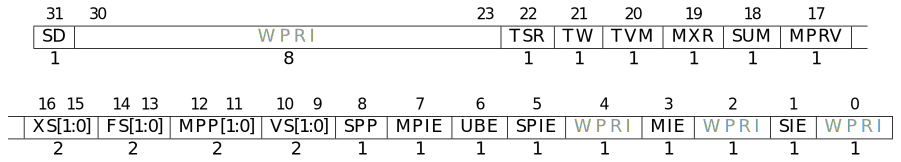
\includegraphics[width=0.95\textwidth]{riscv-mstatus.pdf}
\end{center}

\begin{tabular}{|l|l|l|}  \hline
Field & Bit(s) & Description/Use \\\hline
SIE & 1 & Supervisor global interrupt enable \\\hline
MIE & 3 & Machine global interrupt enable (for handler atomicity) \\\hline
SPIE & 5 & SIE (previous) before trapping to system mode \\\hline
MPIE & 7 & MIE (previous) before trapping to machine mode \\\hline
SPP & 8 & Priority mode before trapping to system mode \\\hline
VS & 10:9 & Inform if floating point save is needed \\\hline
MPP & 12:11 & Priority before trapping into machine mode \\\hline
\end{tabular}
\end{frame}

\begin{frame}
\frametitle{RISC-V -- Exception/Interrupt Cause Register}

Machine Cause Register -- \textbf{mcause}

\begin{center}
  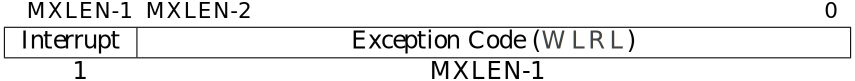
\includegraphics[width=0.95\textwidth]{riscv-mcause.pdf}
\end{center}

\small
The register informs the handler about the source of the exception, the interrupt.

If the most significant bit is set (RV32 bit 31, RV64 bit 63), then the source is an asynchronous exception/peripheral/external interrupt. The exception code corresponds to the source and the corresponding enable and pending source bit positions in the registers \textbf{mie} and \textbf{mip}. \textbf{mepc} points to the interrupted (first unprocessed) instruction. Finalization of the routine by \textbf{mret} instruction will transfer execution of the interrupted program from its next instruction. When the most significant bit is zero, the exception is a synchronous source. \textbf{mepc} points to the instruction that caused it. If the cause (e.g. page fault) is resolved, the instruction will be re-executed simply after \textbf{mret} returns. If the reason is a system call (ecall instruction), \textbf{ebreak} or \textbf{ebreak} or \textbf{ebreak} or invalid instruction that is emulated by the handler, then it is necessary to move \textbf{mepc} after the instruction that caused the exception before returning \textbf{mret}

\end{frame}

\begin{frame}
\frametitle{RISC-V -- Coding of Causes of Synchronous Exceptions}

\begin{center}
\small
\begin{tabular}{|l|l|l|}  \hline
External (IRQ) & Number & Cause/Source \\\hline
0 & 0 &Instruction address misaligned \\\hline
0 & 1 & Instruction access fault \\\hline
0 & 2 & Illegal instruction \\\hline
0 & 3 & Breakpoint exception \\\hline
0 & 4 & Load address misaligned \\\hline
0 & 5 & Load access fault \\\hline
0 & 6 & Store/AMO address misaligned \\\hline
0 & 7 & Store/AMO access fault \\\hline
0 & 8 & Environment call from U-mode \\\hline
0 & 9 & Environment call from S-mode \\\hline
0 & 11 & Environment call from M-mode \\\hline
0 & 12 & Instruction page fault \\\hline
0 & 13 & Load page fault \\\hline
0 & 15 & Store/AMO page fault \\\hline
0 & 24...31 &Designated for custom use \\\hline
\end{tabular}
\end{center}
\end{frame}

\begin{frame}
\frametitle{RISC-V -- Coding of Causes of Asynchronous Interrupts}

\begin{center}
\small
\begin{tabular}{|l|l|l|}  \hline
External (IRQ) & Number & Cause/Source \\\hline
1 & 1 & Supervisor software interrupt \\\hline
1 & 3 & Machine software interrupt \\\hline
1 & 5 & Supervisor timer interrupt \\\hline
1 & 7 & Machine timer interrupt \\\hline
1 & 9 & Supervisor external interrupt \\\hline
1 & 11 & Machine external interrupt \\\hline
1 & $\ge$16  & Designated for platform use \\\hline
\end{tabular}
\end{center}

\small
Register \textbf{mie} enables individual interrupt sources, bit position corresponds to
source

Register \textbf{mip} informs about currently pending/pending resources

\textbf{mstatus.MIE} global enable (1) / disable (0)

There is another set of registers for system mode control

\textbf{sstatus}, \textbf{sie}, \textbf{sip}, \textbf{sscratch}, \textbf{scause} etc. Their structure is
the same/similar, but they are accessible from system mode (supervisor) when access to machine mode registers is not allowed

\end{frame}

\begin{frame}
\frametitle{RISC-V -- Exception/Interrupt Processing}

CPU accepts interrupt request, exception or \textbf{ecall} opcode (either in user, system, or machine mode)

\begin{itemize}
 \item mepc <= pc and switches to machine privilege mode
 \item mstatus.MPP and mstatus.MPV set to preceding privilege mode
 \item mcause <= exception code, mcause[XLEN-1] <= 1 if interrupt
 \item mstatus.MPIE <= mstatus.MIE, mstatus.MIE <= 0
 \item PC <= mtvec (for vectored mode and interrupts BASE+4×cause)
\end{itemize}

The prolog of IRQ/service handler is responsible for determining
the cause \texttt{csrr rd, mcause} and saving of the rest of
the state which could be inadvertently modified

The processor state is obtained and controlled via control and status registers -- CSR

\begin{tabular}{l c l}
\multicolumn{2}{l}{\texttt{csrrw rd, csr, rs1}} & \texttt{csrrwi rd, csr, uimm5} \\
\multicolumn{2}{l}{\texttt{csrr(s/c) rd, csr, rs1}}  & \texttt{csrr(s/c)i rd, csr, uimm5} \\
\texttt{csrr rd, csr} &  $=$ & \texttt{csrrs rd, csr, x0} \\
\texttt{csrw csr, rs1} & $=$ & \texttt{csrrw x0, csr, rs1} \\
\end{tabular}
\end{frame}

\begin{frame}
\frametitle{RISC-V -- Exception/Interrupt Processing Finalization}

The service routine informs by insertion/execution of \textbf{mret} opcode (from system mode \textbf{sret})
CPU that exception/interrupt handling has finished and saved state should be restored, usually original
mode and program

\begin{itemize}
 \item priviledge mode from mstatus.MPP and mstatus.MPV
 \item mstatus.MPV <= 0, mstatus.MPP <= 0
 \item mstatus.MIE <= mstatus.MPIE
 \item pc <= mepc and continue execution in mode restored from mstatus.MPP
\end{itemize}
\end{frame}

\begin{frame}
\frametitle{Precise Exception Handling}

If the interrupt/exception is successfully handled (i.e., the missing page
has been swapped in, etc.), then execution continues
with the causing instruction (at which the exception was received).
The flow of the interrupted code is not changed and from the perspective
of the program it is not possible to detect that the problem has occurred
(except for delays/timing and cases when the modification of the state
is intended/caused by the handling of system calls)

\vspace{3mm}

Note: Precise exception handling is complicated the most by delayed
writes (changing the order of execution of instructions on superscalar
architectures). This leads to the detection of synchronous exceptions
even many instructions later. The concept of rollback or confirmation
of "transactions" is then necessary to allow memory paging, etc.

\end{frame}

\begin{frame}
\frametitle{Evaluation of the Exception Sources on RISC-V}

\begin{itemize}
 \item Software cause evaluation (sometimes polled exception handling)
 \begin{itemize}
  \item All exceptions/interrupts start same service routine at same
   address -- i.e. for RISC-V $PC$ is set to mtvec \textbf{mtvec}. \textbf{stvec}
   for supervisor mode.
  \item Routine reads cause from status register (RISC-V: \textbf{mcause} Registrovat)
 \end{itemize}
 \item Vectored Exception Handling (usually not used on RISC-V)
 \begin{itemize}
  \item Identification of the cause source in the cause/source/interrupt numbers
   in the processor hardware
  \item The table of service routines start addresses starts at fixed
   or configurable address (VBR -- vector base register) in main memory
  \item CPU uses cause number as an index into the table
  \item CPU loads the word/service rutine start into $PC$
 \end{itemize}
 \item Non-vectored exception handling with multiple routines/start
      addresses assigned to exception classes and/or interrupt priorities
\end{itemize}

\footnotesize

On RISC-V, evaluation either purely in software, the routine from~\textbf{mtvec} or if \textbf{mtvec}.0=1, then \textbf{mtvec} points to the table start, then at position zero a reference to the (external) interrupt handler, and entries for individual synchronous exceptions follows.
\end{frame}

\begin{frame}[fragile]
\frametitle{Exception Service Routine Example – Setup}

\begin{columns}
\begin{column}{0.5\textwidth}
\begin{minted}[fontsize=\footnotesize]{gas}
_start:
   addi   a0, zero, 0x101
   la     t0, skip
   csrrw  zero, mepc, t0
   mret   # test exception ret
   addi   a0, zero, 0x105
   addi   a0, zero, 0x106
skip:
   addi   a0, zero, 0x107
   csrrs  t0, mepc, zero
   ebreak
   la     t0, handle_exception
   csrrw zero, mtvec, t0
   la     t0, task_control_block
   csrrw zero, mscratch, t0
   csrrsi zero,mstatus,8 # MIE=1
   addi t0, zero, 16 # UART RX
   addi t1, zero, 1
   sll t1, t1, t0 # bit mask
\end{minted}
\end{column}
\begin{column}{0.5\textwidth}
\begin{minted}[fontsize=\footnotesize]{gas}
   csrrs zero, mie, t1
   li   a0, SERIAL_PORT_BASE
   li   t0, SERP_RX_ST_REG_IE_m
   sw   t0, SERP_RX_ST_REG_o(a0)
   # Background task
   addi t0, zero, 0x0001
   li   a0, SPILED_REG_BASE
Loop:
   csrrs t1, mepc, zero # check
   sw   t1,SPILED_REG_LED_LINE(a0)
   srl t2, t0, 31
   sll t0, t0, 1
   or   t0, t0, t2
   lw   t2, ..._KNOBS_8BIT(a0)
   sw   t2, ..._LED_RGB1(a0)
   xori t2, t2, -1
   sw   t2, ..._LED_RGB2(a0)
   beq zero, zero, loop
\end{minted}
\end{column}
\end{columns}

\end{frame}

\begin{frame}[fragile]
\frametitle{Exception Service Routine Example -- Interrupts Processing}

\begin{minted}[fontsize=\footnotesize]{gas}
handle_exception:
    csrrw   tp, mscratch, tp      # store previous and take system tp
    sw      sp, TCB_SP(tp)        # store stack pointer
    sw      ra, TCB_RA(tp)        # store return address
    sw      t0, TCB_T0(tp)        # store rest of clobberable regs
    sw      a0, TCB_A0(tp)
    ...
    csrr    t0, mcause            # is it Rx interrupt?
    blt     t0, zero, handle_irq  # branch to interrupts processing
    ...
    # handle synchronous exception
ret_from_exception:
    lw      sp, TCB_SP(tp)        # restore stack pointer
    lw      ra, TCB_RA(tp)        # restore return address
    lw      t0, TCB_T0(tp)        # restore rest of clobberable regs
    lw      a0, TCB_A0(tp)
    ...
    csrrw   tp, mscratch, tp      # Swap back TCB to mscratch
    mret                          # Return from exception pc <= mepc
\end{minted}
\end{frame}

\begin{frame}[fragile]
\frametitle{Exception Service Routine Example -- Serial Port Echo}

\begin{minted}[fontsize=\footnotesize]{gas}
handle_irq:                        # t0 mcause
    slli    t0, t0, 2              # shift out sign, left sources * 4
    # the t0 would be used to point into irq handlers table
    # check only for UART RX interrupt for simplicity 8
    addi    a0, zero, 16 * 4       # UART RX is the first platform irq
    beq     t0, a0, handle_uart_rx_irq # it is UART RX
    # mask out unknown sources
    srli    t0, t0, 2              # make t0 back simple source index
    addi    a0, zero, 1
    sll     a0, a0, t0             # generate bit mask for source
    csrrc   zero, mie, a0          # mie = mie & ~a0
    j       ret_from_exception
handle_uart_rx_irq:
    li      a0, SERIAL_PORT_BASE   # Setup base of UART
    lw      t0, SERP_RX_DATA_REG_o(a0) # Read received character
    sw      t0, SERP_TX_DATA_REG_o(a0) # echo it back to terminal
    j       ret_from_exception
\end{minted}

\tiny

\url{https://gitlab.fel.cvut.cz/b35apo/stud-support/-/blob/master/seminaries/qtrvsim/uart-echo-irq/uart-echo-irq.S}

QtRVSim, the RISC-V simulator (QtMips for MIPS) already supports exceptions processing

\end{frame}

\begin{frame}
\frametitle{Interrupts -- Operating Systems Level I/O Processing}

When the application is waiting for incoming data or for space to send next one, the task is suspended/waiting (the processor can serve another tasks). After receiving the data, the peripheral
informs the processor with an interrupt and it completes the transfer and releases
the original task to continue

\begin{center}
  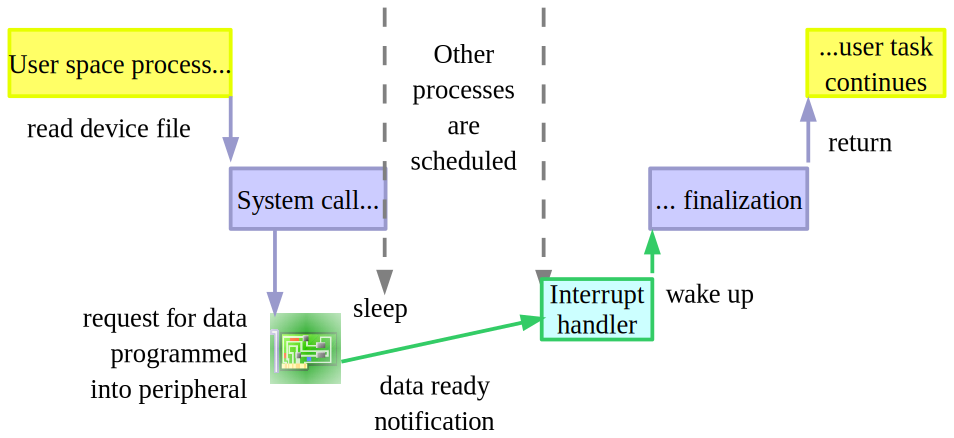
\includegraphics[width=0.94\textwidth]{irq-and-os-intercation.pdf}
\end{center}

\tiny

Source: bootlin: Kernel, drivers and embedded Linux development \url{https://bootlin.com/}

\end{frame}

\section{Direct Memory Access -- DMA}

\begin{frame}
\frametitle{Direct Access to Memory from Peripherals or by DMA Controller}

\begin{itemize}
\item The processor sets the peripheral and the memory address from which/where the data should be transferred
\item Then the I/O operation is started by CPU in peripheral and either the peripheral
 directly accesses the main memory or requests a centra direct memory access (DMA)
 controller via a DRQ
\item For classic shared buses, it is necessary to ensure that for each data
 transfer, cycle, the bus control is released by the central element, the CPU,
 and the address selection and the data transfer control is performed by
 the peripheral or the central DMA controller
\item After transferring the specified number of bytes, the processor is informed
 about the completion of the transfer (or about an error that occurred)
 by the interrupt mechanism
\end{itemize}

\end{frame}

\begin{frame}
\frametitle{Direct memory Access -- Disk Read, Step 1}

\begin{center}
  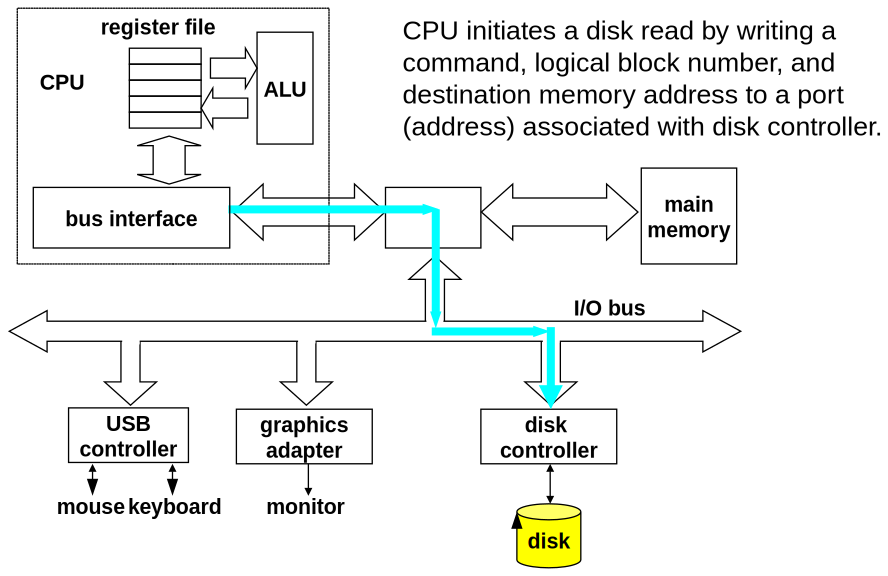
\includegraphics[width=0.90\textwidth]{dma-transfer-1.pdf}
\end{center}

\end{frame}


\begin{frame}
\frametitle{Direct memory Access -- Disk Read, Step 2}

\begin{center}
  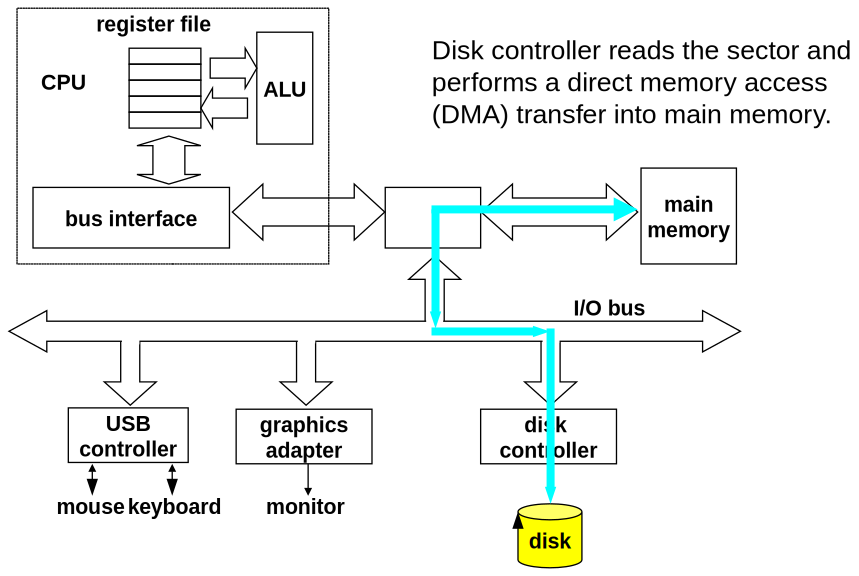
\includegraphics[width=0.90\textwidth]{dma-transfer-2.pdf}
\end{center}

\end{frame}

\begin{frame}
\frametitle{Direct memory Access -- Disk Read, Step 3}

\begin{center}
  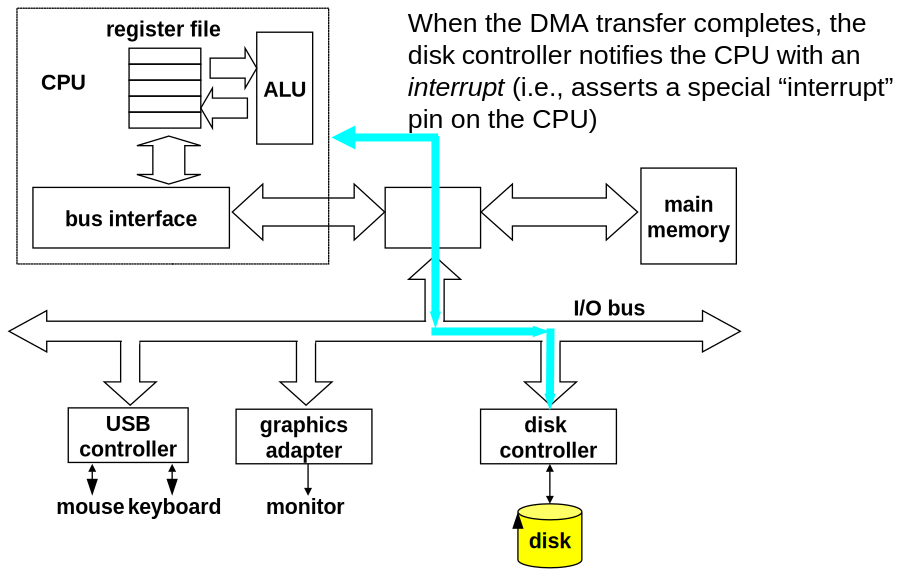
\includegraphics[width=0.90\textwidth]{dma-transfer-3.pdf}
\end{center}

\end{frame}

\section{Consequences of Using Cache Memories, Out-of-Order Execution, Multiple Cores}

\begin{frame}
\frametitle{Cache Memories, Multiple Cores and Memory Accesses}

\begin{itemize}
\item When accessing memory outside a given processor core, it is necessary to take into account that data may be located in cache memories at different levels of the memory hierarchy
\item Access without invalidation, flushing or forwarding would lead to violation of memory coherence rules
\item For most multiprocessor/multicore systems, this is handled by the processor hardware, at least between threads
\item Coherence during transfers from/to peripherals is handled differently on different architectures and their implementations. For ranges intended for receiving and sending data, the operating system must
call functions that guarantee synchronization or invalidation of the range in cache memories
before starting the transfer to the peripherals (as required on the given architecture).

\begin{itemize}
\item  on the x86 architecture, these functions are usually empty or contains only a barrier for synchronization of the processor core itself
\item on ARM, it is necessary to issue instructions to flush/invalidate the buffer with step/span of cache line size.
\end{itemize}
\end{itemize}
\end{frame}

\begin{frame}[fragile]
\frametitle{Out-of-order Instruction Execution and Memory Barriers}

\begin{itemize}
\item Assume that the coherence of individual memory locations is guaranteed, either in hardware or for peripherals in software
\item However, if the processor executes instructions out of order, then memory accesses order can be permuted
\item problem to prevent, an instruction to start a transfer writes data to a command register before the target address is set
\item Similarly, a thread on the other processor can confirm by writing to memory that data is ready at another address but the write instructions are not completed
\item The compiler can also arbitrarily rearrange the order of accesses or skip repeated stores but the last one to given address

\end{itemize}

\end{frame}

\begin{frame}[fragile]
\frametitle{Out-of-order Instruction Execution and Memory Barriers}

\begin{itemize}
 \item It is therefore necessary to define sequence points where no (or only certain) accesses can be moved forward and further in execution order. Such constructs are defined for each language, runtime environment
and realized by specialized instructions at the processor level. For example, on MIPS \textbf{sync}, on RISC-V \textbf{fence} on x86 overload of already existing intructions is used. To insert a barrier from GCC on x86
\end{itemize}

\begin{minted}[fontsize=\footnotesize]{c}
asm volatile("lock; addl $0,-4(%%esp)" ::: "memory", "cc")
\end{minted}

\begin{itemize}
\item The newer x86 generations with SSE2 support provide
\end{itemize}

\texttt{mfence}, \texttt{lfence} a \texttt{sfence}

\begin{itemize}
\item The base for more complex atomic operations is \textbf{Compare and Swap}, on x86:
\end{itemize}

\begin{minted}[fontsize=\footnotesize]{c}
__asm__ volatile ("xchgl %0,%1" :"=r" (x) :"m" (y), "0" (x) :"memory");
\end{minted}
\end{frame}

\end{document}

